\documentclass[11pt]{beamer}
\usepackage[utf8]{inputenc}
\usepackage{amsmath}
\usepackage{amsfonts}
\usepackage{amssymb}
\usepackage{graphicx}
\usepackage{ragged2e}
\usepackage{hyperref}
\usepackage{float}
\usepackage{url}
\usepackage{caption} 
\captionsetup{labelformat=empty}
\usetheme{Madrid}
\usecolortheme{default}
\newcommand{\celda}[1]{
	\begin{minipage}{2.5cm}
		\vspace{5mm}
		#1
		\vspace{5mm}
	\end{minipage}
}

\usepackage{tikz}
\usetikzlibrary{shapes.arrows}

\tikzset{
    myarrow/.style={
        draw,
        fill=black,
        single arrow,
        minimum height=5ex,
        single arrow head extend=0.5ex
    }
}

\newcommand{\arrowdown}{%
\tikz [baseline=-1ex]{\node [myarrow,rotate=-90] {};}
}

\newcommand{\arrowright}{%
\tikz [baseline=-1ex]{\node [myarrow,rotate=0] {};}
}

\author[rodrigueznavas@posgrado.uimp.es]{Laura Rodríguez Navas\inst{1}}
\title[Introducción a la Investigación]{A Graphical Tool \\ for the Interpretation of Medical Data}
\date{May 2020} 
\logo{
\includegraphics[scale=0.0375]{img/logo.jpg}}
\institute[UIMP]{
	\inst{1}
		Universidad Internacional Menéndez Pelayo (UIMP) \\Máster Universitario en Investigación en Inteligencia Artificial \\ 
}

\AtBeginSection[]
{
	\begin{frame}<beamer>{Content}
		\tableofcontents[currentsection,currentsubsection]
	\end{frame}
}

\begin{document}
	
\begin{frame}
	\maketitle
\end{frame}

\begin{frame}{Content}
	\tableofcontents
\end{frame}

\section{Procedure}
	\begin{frame}{Procedure}
		\begin{block}{}
		\centering
        Dataset \\
        \vspace{0.3cm}
        \arrowdown\\[0.5ex]
        Gaifman Graph \\ (several variations) \\
        \vspace{0.3cm}
        \arrowdown\\[0.5ex]
        Clan Decomposition Method
        \end{block}
	\end{frame}

\section{Hospitalization Dataset}
	\begin{frame}{Hospitalization Dataset}
	    \begin{figure}
	        \centering
	        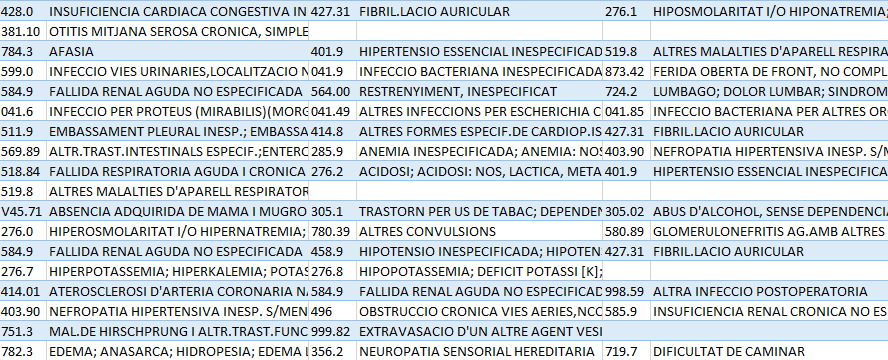
\includegraphics[width=1 \linewidth]{img/table.png}
	    \end{figure}
	\end{frame}

\section{Clan Decomposition Method}
	\begin{frame}{Clan Decomposition Method}
	    \begin{columns}
            \begin{column}{0.4\textwidth}
                \begin{figure}
                    \centering
                    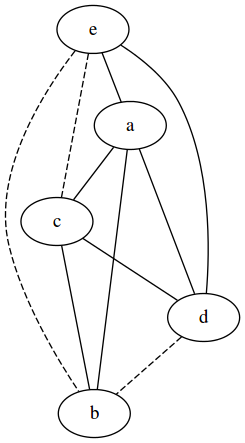
\includegraphics[width=0.6 \textwidth]{img/exampleasycomp.png}
                \end{figure}
            \end{column}
            
            \begin{column}{0.2\textwidth}
                \centering
                \arrowright\\[0.5ex]
                \begin{table}
                \caption{Patients}
                \vspace*{-\baselineskip}
                    \begin{tabular}{ c  c  c  c }
                        p1: & a & b & c \\ 
                        p2: & a & d & e \\  
                        p3: & a & c & d   
                    \end{tabular}
                \end{table}
            \end{column}
            
            \begin{column}{0.4\textwidth}
            \begin{figure}
                \centering
                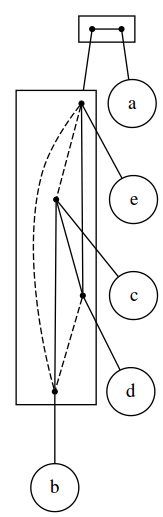
\includegraphics[width=0.4 \textwidth]{img/exampleasydecomp.png}
                \end{figure}
            \end{column}
        \end{columns}
	\end{frame}

\section{Hospitalization Graph Decomposition}
	\begin{frame}{Hospitalization Graph Decomposition}
		\begin{columns}
        \column{0.4\textwidth}
            \begin{figure}
                \centering
                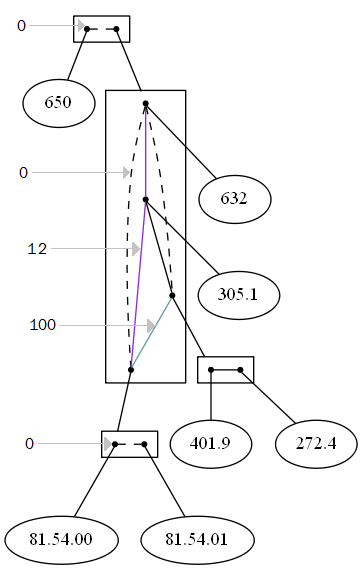
\includegraphics[width=0.9 \textwidth]{img/datahsp_withoutV_100_exp_values_conected_1.png}
            \end{figure}
         
        \column{0.5\textwidth}
            \begin{itemize}
                \item 650 Normal delivery.
                \item 632 Missed abortion.
                \item 305.1 Tobacco use disorder.
                \item 401.9 Unspecified essential hypertension.
                \item 272.4 Other and unspecified hyperlipidemia.
            \end{itemize}
        \end{columns}
	\end{frame}

\section{Conclusions}
	\begin{frame}{Conclusions}
		\begin{block}{Purpose}
        To be an exploratory tool from data.
        \end{block}
        
        \begin{block}{After the analysis...}
            \begin{itemize}
                \item To have a general view about co-occurring diagnostics.
                \item To complement statistical approaches.
            \end{itemize}
        \end{block}
	\end{frame}

\begin{frame}
    \Huge{\centerline{\textbf{THANK YOU!}}}
\end{frame}

\end{document}